\par The Raspberry Pi 3 Model A+ is the latest product in the Raspberry Pi 3 range, weighing in at just 29 g. Like the Raspberry Pi 3 Model B+, it boasts a 64-bit quad core processor running at 1.4 GHz, dual-band 2.4 GHz and 5 GHz wireless LAN, and Bluetooth 4.2/BLE. The dual-band wireless LAN comes with modular compliance certification, allowing the board to be designed into end products with significantly reduced wireless LAN compliance testing, improving both cost and time to market. The Raspberry Pi 3 Model A+ has the same mechanical footprint as the older Raspberry Pi 1 Model A+.
	\begin{figure}[h]
		\centering
		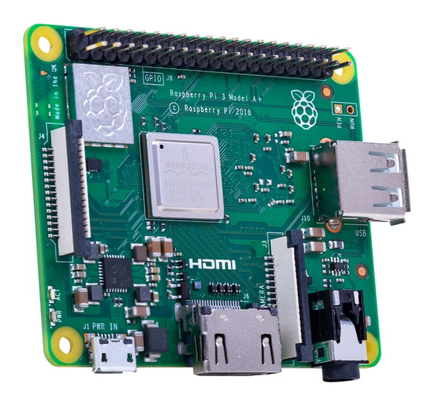
\includegraphics[width=3in]{rasPi.png}
		\caption{Raspberry Pi 3 Model A+}
	\end{figure}
\subsubsection{Raspberry Pi Camera (Hardware and Software)}
\begin{figure}[h]
	\centering
	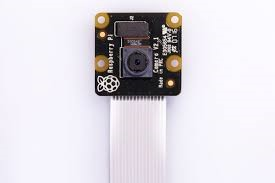
\includegraphics[width=2in]{picam.jpg}
	\caption{Pi NOIR Camera unit}
\end{figure}
\par The Raspberry Pi Camera v2 is the new official camera board released by the Raspberry Pi Foundation. The Raspberry Pi Camera Module v2 is a high quality 8 megapixel Sony IMX219 image-sensor custom designed add-on board for Raspberry Pi, featuring a fixed focus lens. It's capable of 3280 x 2464 pixel static images, and also supports 1080p30, 720p60 and 640x480p90 video. It attaches to Pi by way of one of the small sockets on the board upper surface and uses the dedicated CSi interface, designed especially for interfacing to cameras.

\subsubsection{PyAudio}
\par To begin the raspberry pi will receive a trigger from the Xbee to activate the camera. The camera would then take several pictures or a video file. The goal was to take a video of whoever approached the front door sensed by the motion sensor. The motion sensor would then communicate in tandem with the Xbee device and send a signal to the other Xbee device on the Raspberry Pi. The Xbee is connected to pin 16 on the Raspberry Pi and that will then start the camera to record the person at the door. Once the camera has captured enough video or pictures, the raspberry pi will then send the files to the main computer for viewing through the GUI. 
\par Since the camera component does not work, we are replacing with recording audio whenever pin 16 is activated the code to record the audio via the microphone for whenever a person is at the door will be the main process instead. Through the implementation of python code and the triggers from the Xbee the raspberry pi will record audio of whenever motion is detected at the door and then save an audio file of the encounter which will then be automatically transferred over to the main computer over the network via WinSCP and the use of the planned GUI.


%%%% REMOVED DETAILED LIST OF RASBERRY PI FEATURES	
%	\begin{itemize}
%		\item Processor 
%		\begin{itemize}
%			\item Broadcom BCM2837B0, Cortex-A53
%			\item 64-bit SoC @ 1.4 GHz
%		\end{itemize}
%		\item Memory
%		\begin{itemize}
%			\item 512MB LPDDR2 SDRAM
%		\end{itemize}
%		\item Connectivity
%		\begin{itemize}
%			\item 2.4 GHz and 5 GHz IEEE 802.11.b/g/n/ac wireless LAN
%			\item Bluetooth 4.2/BLE
%		\end{itemize}
%		\item Data and I/O interfacing
%		\begin{itemize}
%			\item Extended 40-pin GPIO header
%		\end{itemize}
%		\item Video and Sound
%		\begin{itemize}
%			\item 1x HDMI
%			\item MIPI DSI display port
%			\item MIPI CSI camera port
%			\item 4 pole stereo output and composite video port
%		\end{itemize}
%		\item Multimedia 
%		\begin{itemize}
%			\item H.264, MPEG-4 decode (1080p30)
%			\item H.264 encode (1080p30)
%			\item OpenGL ES 1.1, 2.0 graphics
%		\end{itemize}
%		\item SD card Support
%		\begin{itemize}
%			\item Micro SD format for loading operating system and data storage
%		\end{itemize}
%		\item Input Power Specifications
%		\begin{itemize}
%			\item 5 V/2.5 A DC via micro USB connector
%			\item 5 V DC via GPIO header
%		\end{itemize}
%	\end{itemize}